\documentclass[11pt,letterpaper]{article}
\usepackage[margin=0.75in]{geometry}
\usepackage{parskip,float,booktabs,tabularx,array,amsmath,amssymb}
\usepackage[T1]{fontenc}
\usepackage{lmodern,microtype,xcolor,tikz}
\usetikzlibrary{arrows.meta,positioning}
\usepackage[hidelinks]{hyperref}
\usepackage{xurl,graphicx,needspace}
\widowpenalty=10000
\clubpenalty=10000
\urlstyle{same}
\definecolor{evidenceblue}{HTML}{245B83}
\definecolor{decisiongreen}{HTML}{28604A}
\definecolor{reviewamber}{HTML}{785217}
\tikzset{flowarrow/.style={-{Latex[length=2mm]},line width=.75pt},panel/.style={draw=evidenceblue,fill=evidenceblue!4,rounded corners=2pt,align=left,inner sep=8pt,font=\small}}
\newcolumntype{Y}{>{\raggedright\arraybackslash}X}
\newcommand{\run}[1]{\texttt{\detokenize{#1}}}
\setlength{\emergencystretch}{2em}
\setlength{\extrarowheight}{1pt}
\setlength{\parskip}{5pt plus 1pt}
\setlength{\intextsep}{8pt plus 1pt}
\setlength{\abovecaptionskip}{5pt}
\setlength{\belowcaptionskip}{0pt}
\hypersetup{pdftitle={Pairwise Preferences and Citation Evidence for TREC AutoJudge 2026},pdfauthor={Nidhin Pattaniyil and Tanwir Zaman}}
\begin{document}
\begin{center}
{\Large\bfseries Pairwise Preferences and Citation Evidence\\for TREC AutoJudge 2026\par}
\vspace{8pt}Nidhin Pattaniyil \quad Tanwir Zaman\\Team: ntp
\end{center}
\section*{Abstract}
We describe three submitted methods for judging answers from the RAG and RAGTIME tracks. \textbf{Pairwise} asks which of two answers is better. \textbf{Evidence} checks whether an answer covers the question and whether its citations support its claims. \textbf{Combined} averages the two scores.

We submitted all three approaches to both tracks. Pairwise uses ten opponents per answer and compares both presentation orders. Evidence uses one shared checklist per question, separate coverage and citation judgments, and half credit for partial support. Combined gives the two scores equal weight. This paper describes these final submissions.

\section{One task, three approaches}
RAG and RAGTIME systems generate answers with citations to source documents. AutoJudge evaluates those answers and predicts a leaderboard~\cite{autojudge}. Our output is a score for each system. The organizer later evaluates how well the predicted ranking matches the host track's assessment.
\begin{figure}[H]\centering
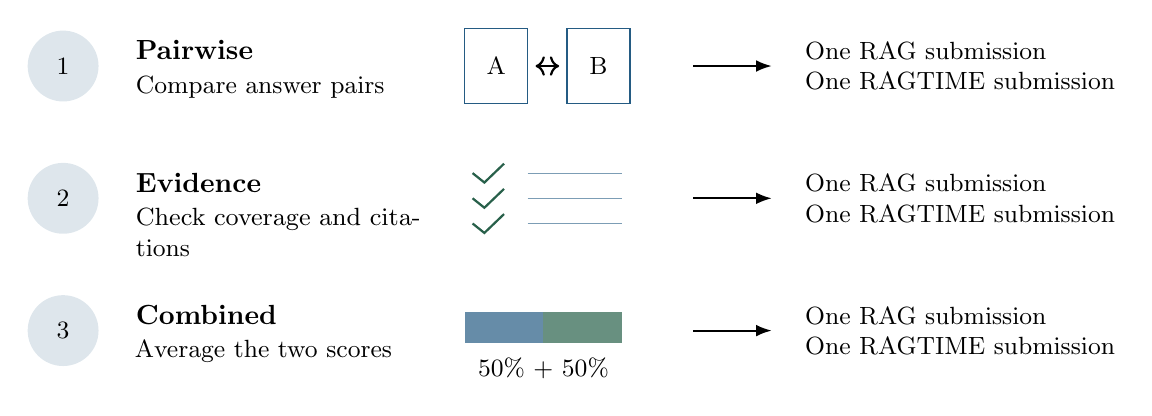
\begin{tikzpicture}[font=\small,y=.8cm]
\foreach \y/\num/\title/\desc in {0/1/Pairwise/{Compare answer pairs},-2.1/2/Evidence/{Check coverage and citations},-4.2/3/Combined/{Average the two scores}} {
\node[circle,fill=evidenceblue!15,minimum size=9mm] at (0,\y) {\num};
\node[anchor=west,font=\bfseries] at (.8,\y+.25) {\title};
\node[anchor=north west,align=left,text width=3.6cm,inner ysep=0pt] at (.8,\y-.15) {\desc};
\draw[flowarrow] (8,\y)--(9,\y);
\node[anchor=west,align=left] at (9.3,\y) {One RAG submission\\One RAGTIME submission};}
\foreach \x/\lab in {5.5/A,6.8/B} {\draw[evidenceblue] (\x-.4,.6) rectangle (\x+.4,-.6);\node at (\x,0) {\lab};}
\draw[<->,thick] (6,0)--(6.3,0);
\foreach \y in {-1.7,-2.1,-2.5} {\draw[decisiongreen,thick] (5.2,\y)--(5.35,\y-.15)--(5.6,\y+.15);\draw[evidenceblue!60] (5.9,\y)--(7.1,\y);}
\fill[evidenceblue!70] (5.1,-3.9) rectangle (6.1,-4.4);
\fill[decisiongreen!70] (6.1,-3.9) rectangle (7.1,-4.4);
\node at (6.1,-4.8) {50\% + 50\%};
\end{tikzpicture}
\caption{Three judging approaches, each submitted to both tracks: six submissions in total. Pairwise and Evidence can be used independently; Combined averages their scores.}
\end{figure}
\textbf{Scope.} We submitted each method to both tracks, giving six submissions. For RAG, our judges scored answers from 83 submitted systems across 119 questions. For RAGTIME, they scored answers from 49 systems across 103 questions. Here, a system is an answer-generation run being judged, not one of our three judging methods.

\textbf{Coverage and support.} An answer can mention everything requested and still cite weak evidence. We use a four-day-workweek example to show why we keep those judgments separate.

\clearpage
\section{Pairwise: compare, swap, then fit a ranking}
The judge sees the question and two answers, including their citation markers. It returns a winner or a tie. Comparing both orders reduces sensitivity to answer position~\cite{wang,zheng}; it cannot guarantee a correct judgment.

\textbf{Workweek example} (illustrative, inspired by RAGTIME 2025 topic 1033).
\begin{center}
\begin{tabularx}{\linewidth}{@{}lY@{}}\toprule
Question & How does a four-day workweek change hours and wellbeing?\\
Answer A & Employees work 32 hours a week [1]. This reduces stress and doubles company profits [2].\\
Answer B & A four-day workweek gives employees more time off.\\\bottomrule
\end{tabularx}
\par\vspace{9pt}
\begin{tabular}{lll}\toprule
Presentation & Assumed decision & Credit to A\\\midrule
A then B & A wins & 1\\
B then A & Tie & .5\\\bottomrule
\end{tabular}
\quad A's pair credit: $(1+.5)/2=\mathbf{.75}$
\end{center}
The answers, sources and votes are authored examples. Preference alone does not establish support for A's profit claim.

\Needspace{16\baselineskip}
\subsection*{From comparisons to a system score}
\begin{figure}[H]\centering
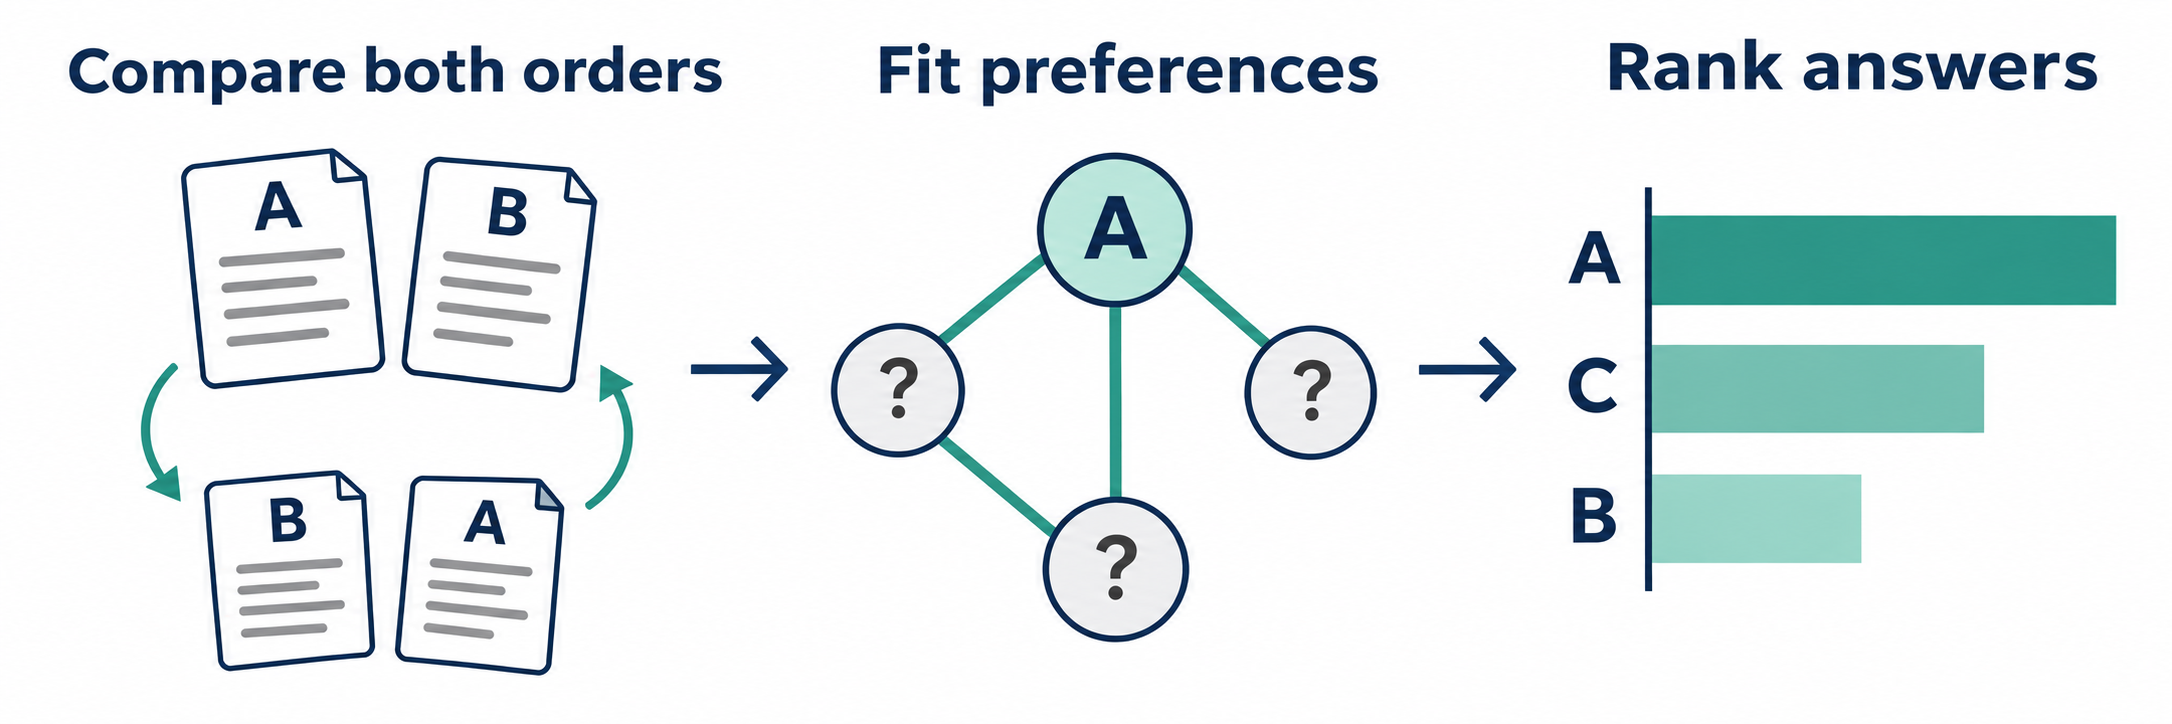
\includegraphics[width=.76\linewidth]{figures/pairwise-generated.png}
\par\medskip
\textbf{Select ten opponents for each answer}
\par\smallskip
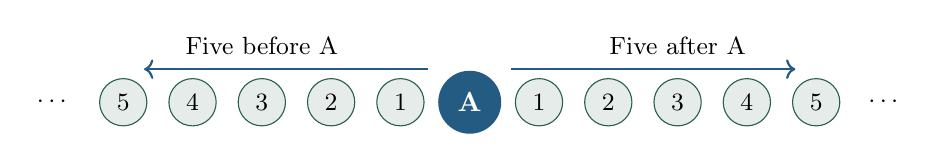
\begin{tikzpicture}[x=.88cm,y=.6cm,font=\small]
\foreach \i in {-5,-4,-3,-2,-1,1,2,3,4,5} {
\node[circle,draw=decisiongreen,fill=decisiongreen!12,minimum size=6mm,inner sep=1pt] at (\i,0) {\pgfmathparse{int(abs(\i))}\pgfmathresult};}
\node[circle,fill=evidenceblue,text=white,minimum size=8mm,font=\bfseries] at (0,0) {A};
\draw[<-,thick,evidenceblue] (-4.7,.7)--(-.6,.7);
\draw[->,thick,evidenceblue] (.6,.7)--(4.7,.7);
\node at (-3,1.2) {Five before A};
\node at (3,1.2) {Five after A};
\node at (-6,0) {$\cdots$}; \node at (6,0) {$\cdots$};
\end{tikzpicture}
\par
For each question, its answers form a fixed hash-ordered ring, shown unrolled above. Numbers mark neighbor distances, not ranks. Repeat for every answer; judge each selected pair in both orders.
\par\medskip
\begin{minipage}[t]{.47\linewidth}\raggedright
\textbf{Fit Bradley--Terry}\\
For each question, fit answer strengths to the votes. Predict win chances against all its answers, including unjudged opponents.
\end{minipage}\hfill
\begin{minipage}[t]{.47\linewidth}\raggedright
\textbf{Average twice}\\
Average each answer's win chances against the other answers. Then average its system's answer scores across questions.
\end{minipage}
\par\vspace{3pt}
\caption{From a limited comparison budget to a full ranking. The question marks represent other anonymous answers. The network and bars illustrate the method, not measured results. Scores estimate preference, not factual correctness.}
\end{figure}
\clearpage
\section{Evidence: check the claim, not just the citation marker}
The evidence branch builds one question-guided checklist from pooled evidence and freezes it for all answers. It then checks coverage separately from support. Our submitted model identifier is \run{openai/gpt-6-luna}; we did not train a new judge.

\begin{figure}[H]\centering
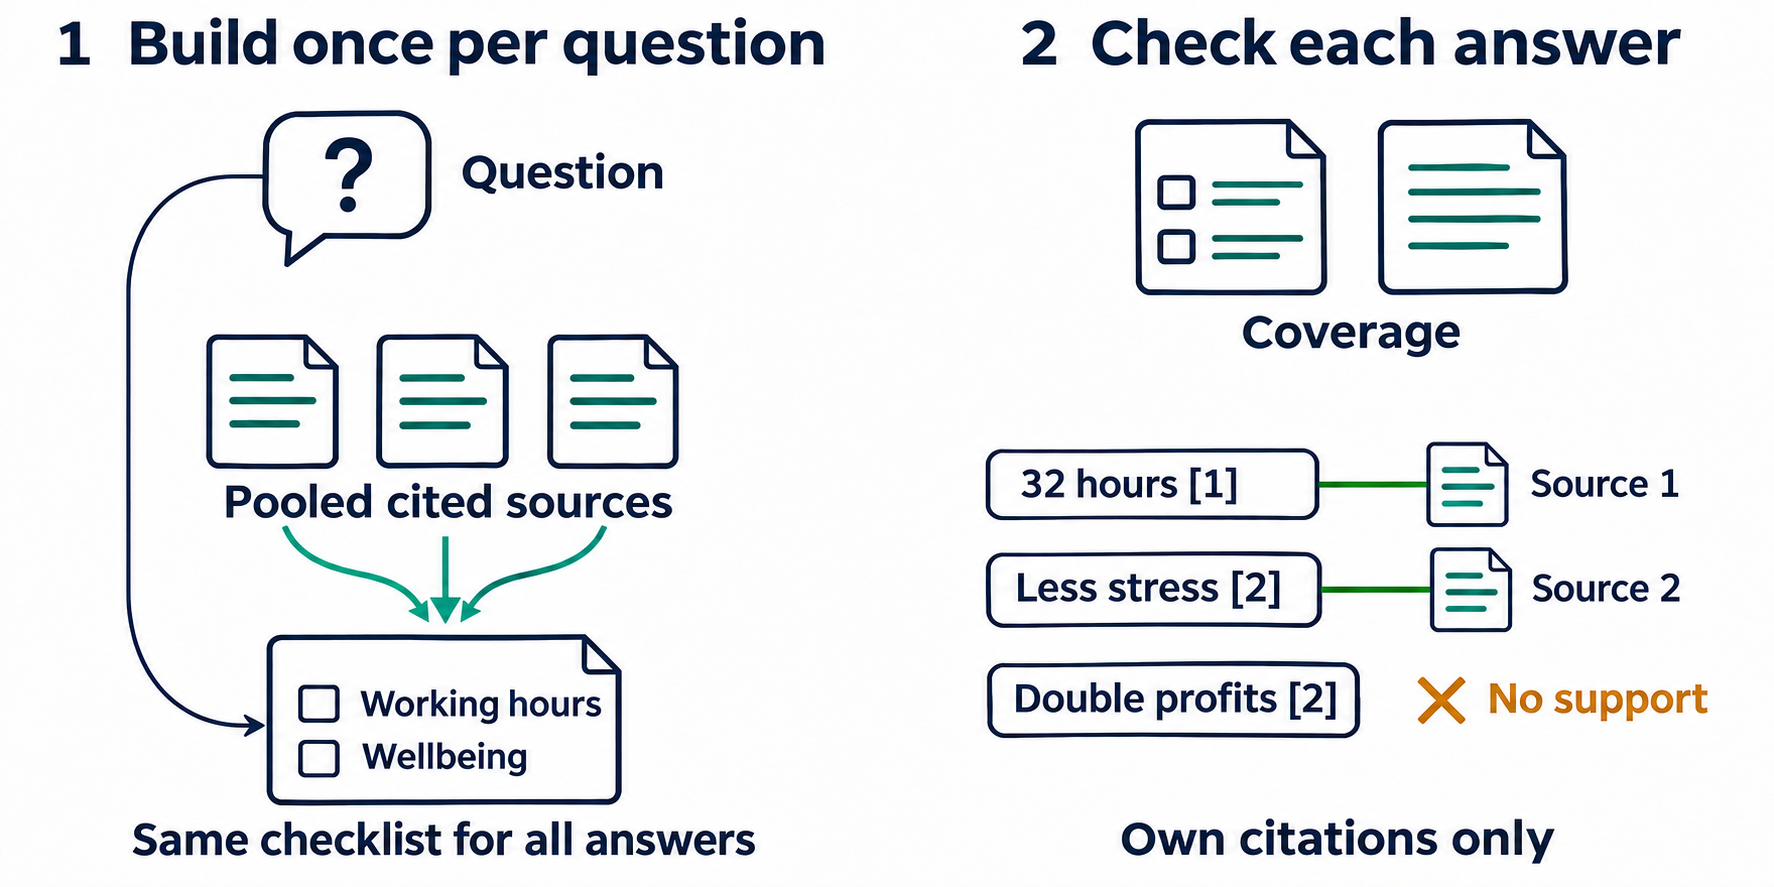
\includegraphics[width=.68\linewidth]{figures/evidence-side-by-side.png}
\caption{Left: the question and pooled cited sources jointly produce a checklist shared by all answers. Right: coverage and own-citation support are judged separately, then linked by segment ID. Stress and profits share one answer segment but are shown separately to reveal partial support.}
\end{figure}

\textbf{Build the checklist once.} The full question and pooled source excerpts guide its requirements. Each item records acceptable alternatives. Required items must be covered; optional items add useful detail. Factual items ask for information, while request-only items concern how the answer should respond. If excerpts exceed the input budget, we use deduplicated, validated claims with provenance and retain qualifications on partial claims.

\textbf{Evaluate each answer.} The coverage judge sees the checklist and answer, but no source text or citation-support labels. A separate citation judgment checks the answer against its own sources. We join these judgments by segment ID and identify the supported portion of a partial claim before assigning grounded coverage.

Coverage measures whether required checklist items are addressed, including factual and request-only items. Grounded factual coverage counts required factual items supported by the answer's own citations. Sources used to build the shared checklist cannot repair a missing or weak citation in that answer. The checklist can still miss important facts.

\subsection*{From judgments to an Evidence score}
Each answer receives a coverage score and citation-support scores, all on a 0--1 scale. We combine them with equal weights:
\par\vspace{4pt}
\[
 E_{\mathrm{RAG}}=\frac{\text{coverage}+\text{citation precision}+\text{citation recall}}{3}
\]
\[
 E_{\mathrm{RAGTIME}}=\frac{\text{grounded factual coverage}+\text{top-citation support}}{2}.
\]
Section~\ref{sec:track-scores} defines these components and explains the different citation rules.

\clearpage
\section{Track-specific scores}\label{sec:track-scores}
RAG evaluates preference, nugget coverage and citation precision/recall~\cite{ragguidelines}. RAGTIME emphasizes correctly cited nuggets and sentence precision~\cite{ragtimeguidelines}. Our shared judgments approximate those targets with two differences:

\begin{center}
\renewcommand{\arraystretch}{1.2}
\begin{tabularx}{\linewidth}{@{}lYY@{}}\toprule
 & \textbf{RAG} & \textbf{RAGTIME}\\\midrule
Coverage & Required checklist items addressed & Required factual items addressed \emph{and supported}\\[5pt]
Citation support & Precision: mean over cited claim--document pairs. Recall: mean of the best single-citation support per segment. & Mean support from each segment's top-priority citation.\\\bottomrule
\end{tabularx}
\end{center}
The Evidence formulas in Section 3 average these components. Optional omissions do not lower coverage.

\subsection*{Same citations, different selection rules}
RAGTIME follows the system's citation priority, as its guidelines require. Our RAG recall uses the best single citation as an approximation; this is our choice, not an organizer rule.

\begin{center}
\renewcommand{\arraystretch}{1.2}
\begin{tabular}{@{}ll@{}}\toprule
\multicolumn{2}{@{}l}{\textbf{Example: one claim, two citations}}\\\midrule
First citation: no support & Second citation: full support\\\midrule
RAG recall: select best $\longrightarrow$ \textbf{1} & RAGTIME: select first $\longrightarrow$ \textbf{0}\\\bottomrule
\end{tabular}
\end{center}

\subsection*{Shared credit rules}
\begin{center}
\begin{tabular}{ccc}
\textcolor{decisiongreen}{\textbf{Full support}} & \textcolor{reviewamber}{\textbf{Partial support}} & \textbf{Unestablished}\\[3pt]
\Large 1 & \Large .5 & \Large 0
\end{tabular}
\end{center}
These credits and the generated checklist are our design choices. Partial citations are not added into full credit; unestablished support does not mean a claim is false.

\begin{center}
\begin{tabularx}{\linewidth}{@{}lY@{}}\toprule
Case & Treatment in both tracks\\\midrule
Uncited segment & Zero citation recall/support.\\
Explicit non-claim & Exclude; retain segments without an explicit label.\\
Empty denominator & Return zero and flag as undefined.\\\bottomrule
\end{tabularx}
\end{center}

\clearpage
\setlength{\extrarowheight}{0pt}
\section{From one answer to a score}
For the illustrative workweek answer, coverage is complete but one citation supports only part of its sentence.

\textbf{1. Coverage: check the two requirements}
\begin{center}
\textcolor{decisiongreen}{$\checkmark$} Working hours \qquad
\textcolor{decisiongreen}{$\checkmark$} Wellbeing
\end{center}
Both requirements are addressed and supported, so both coverage scores are $2/2=\mathbf{1}$. Source [2] supports wellbeing through reduced stress. The answer's unsupported profit claim lowers citation support, not coverage: profits were not requested.

\textbf{2. Citation support: check the two segments (sentences here)}
\begin{center}
\renewcommand{\arraystretch}{1.15}
\begin{tabularx}{\linewidth}{@{}YYr@{}}\toprule
Answer says & Source supports & Credit\\\midrule
``32 hours [1]'' & \textcolor{decisiongreen}{Full:} 32 hours & 1\\[3pt]
``Less stress and double profits [2]'' & \textcolor{reviewamber}{Partial:} less stress only; no support for double profits & .5\\\bottomrule
\end{tabularx}
\end{center}
One citation per sentence makes precision, recall and top-citation support equal here: $(1+.5)/2=\mathbf{.75}$.

\textbf{3. Calculate Evidence, then Combined}
\begin{center}
\renewcommand{\arraystretch}{1.2}
\begin{tabularx}{\linewidth}{@{}lYY@{}}\toprule
 & \textbf{RAG} & \textbf{RAGTIME}\\\midrule
Evidence inputs & Coverage + precision + recall & Grounded coverage + top-citation support\\
Average & $(1+.75+.75)/3=\mathbf{.833}$ & $(1+.75)/2=\mathbf{.875}$\\[5pt]
Add Pairwise & Assume Pairwise $=.60$ & Assume Pairwise $=.60$\\
Combined & $(.60+.833)/2\approx\mathbf{.717}$ & $(.60+.875)/2\approx\mathbf{.738}$\\\bottomrule
\end{tabularx}
\end{center}
Evidence averages \textbf{three components for RAG} and \textbf{two for RAGTIME}. Combined gives Pairwise and Evidence equal weight. The assumed .60 is this answer's fitted Pairwise score for this question, not its .75 credit from one pair. For all three methods, a system's score is the mean of its answer scores across questions.

\subsection*{Submitted runs}
All six runs use \run{openai/gpt-6-luna}. The table gives submission names and data IDs.
\begingroup\small
\begin{center}
\begin{tabularx}{\linewidth}{@{}lYY@{}}\toprule
Method & RAG & RAGTIME\\\midrule
Pairwise & \run{ntp-rag-pairwise-10-v1} (2459) & \run{ntp-ragtime-pairwise-10-v1} (2480)\\
Evidence & \run{ntp-rag-evidence-v1} (2521) & \run{ntp-ragtime-evidence-v1} (2523)\\
Combined & \run{ntp-rag-combined-v1} (2522) & \run{ntp-ragtime-combined-v1} (2524)\\\bottomrule
\end{tabularx}
\end{center}
Frozen revisions: \run{135b5c6} (RAG Pairwise), \run{284040d} (RAGTIME Pairwise), \run{c37a657} (Evidence and Combined). Original judgments are retained for replay.
\endgroup

\Needspace{8\baselineskip}
\begingroup\small\raggedright
\begin{thebibliography}{9}
\bibitem{ragguidelines} TREC RAG organizers. \href{https://github.com/TREC-RAG/trec-rag-skills/blob/main/skills/trec-rag-2026-track-guidelines/references/rag-task.md}{\emph{RAG 2026 task guidelines: Evaluation}}.
\bibitem{ragtimeguidelines} TREC RAGTIME organizers. \href{https://docs.google.com/document/d/1XqypNTHxIdazxfnUebrp-EsUuGNhodhQGrJIDnYGaB4/edit}{\emph{RAGTIME 2026 guidelines: Metrics}}.
\setlength{\itemsep}{0pt}
\bibitem{autojudge} TREC AutoJudge organizers. \href{https://trec-auto-judge.cs.unh.edu/}{\emph{TREC AutoJudge: task and participation information}}.
\bibitem{wang} P. Wang et al. \href{https://arxiv.org/abs/2305.17926}{\emph{Large Language Models are not Fair Evaluators}}. 2023.
\bibitem{zheng} L. Zheng et al. \href{https://arxiv.org/abs/2306.05685}{\emph{Judging LLM-as-a-Judge with MT-Bench and Chatbot Arena}}. 2023.

\end{thebibliography}
\endgroup
\end{document}
